\documentclass[aps,prd,notitlepage,floatfix,superscriptaddress,groupedaddress,nofootinbib]{revtex4-1}
\usepackage{graphicx}  % needed for figures
\usepackage{dcolumn}   % needed for some tables
\usepackage{bm}        % for math
\usepackage{amssymb}   % for math
\usepackage{amsmath}
\usepackage{subcaption}
\usepackage{xcolor}
\usepackage{soul}
\usepackage{natbib}
% \usepackage{booktabs}
\usepackage[singlelinecheck=false, justification=centering]{caption}
\usepackage{listings}
\usepackage{float}
\usepackage{enumitem}
\usepackage{tabularx}
\lstset{basicstyle=\ttfamily,
  showstringspaces=false,
  commentstyle=\color{red},
  keywordstyle=\color{blue}
}

\usepackage{url}
\def\UrlBreaks{\do\/\do-}
\usepackage{breakurl}
\usepackage[breaklinks]{hyperref}

\usepackage[autostyle]{csquotes}

\usepackage[printonlyused, nohyperlinks, withpage]{acronym}

\newcommand{\jscomment}[1]{\colorbox{gray}{\textcolor{yellow}{#1}}}
\newcommand{\jsedit}[2]{\jscomment{\st{#1}}\jscomment{#2}}


\begin{document}

\title{Report on Udacity AI Nanodegree project 3:\\Adversarial search}

\author{Hans-Peter Schadler}
% \affiliation{Austria}

\date{\today}


\begin{abstract}
    In this project we are developing an AI agent for the game Isolation, a fully observable, adversarial and deterministic board game. We will implement the MINIMAX algorithm with Alpha-Beta pruning and analyze the performance of various heuristics for the agent.
\end{abstract}

% \pacs{}
\maketitle

% \tableofcontents

% \newpage

% \makeatletter
% \let\toc@pre\relax
% \let\toc@post\relax
% \makeatother

% \newpage
\section{Problem analysis}

The assignment is to implement a MINIMAX agent (with enhancements like alpha-beta pruning) for the game Isolation and then pick one of three experiments (1. Custom heuristics, 2. Opening book or 3. Advanced search techniques). For this assignment I decided to pick the first topic, developing a custom heuristic and perform various analyses to assess its effectiveness.

All the evaluation runs where performed on a Dell XPS 13 with the following specs:
\begin{itemize}[nosep]
    \item Linux Mint 20.2 Cinnamon
    \item Kernel version 5.14.0-1032-oem
    \item Intel Core i7-1165G7 @ 2.80GHz (4 cores + HT)
    \item 16 GiB memory
\end{itemize}
If not otherwise mentioned, the \textit{run\_search.py} script was always ran with the default time limit of 150ms and with the \textit{fair\_matches.py} option enabled and we always play against the MINIMAX implementation of \textit{sample\_player.py}.

\section{Definition of the heuristics}

In this section, we will define and describe the various heuristics that we tested during this project. For all of the explained heuristics we will show the Python code. The goal was that we use all the possible information that the game functions provide us. These are
\begin{itemize}
    \item Number of possible player moves
    \item Number of possible opponent moves
    \item Play count
    \item Player positions on the board (for example to determine their distance)
\end{itemize}
and we will use various combinations of these in our heuristics.

\subsection{Baseline}
The baseline heuristics is defined by the number of possible player moves - number of opponent moves. It is the heuristics implemented in the sample player MINIMAX algorithm and is implemented also for our custom player in a similar manner. This will serve as the baseline for our comparison.

\begin{lstlisting}[language=python]
def heuristics_liberties(state: Isolation, player: int):
    own_loc = state.locs[player]
    opp_loc = state.locs[1 - player]
    own_liberties = state.liberties(own_loc)
    opp_liberties = state.liberties(opp_loc)
    return len(own_liberties) - len(opp_liberties)
\end{lstlisting}

\subsection*{Liberties: Number of available player moves only}
To define an even simpler heuristics, we use only the number of player moves possible from the current position.

\begin{lstlisting}[language=python]
def heuristics_liberties_player_only(state: Isolation, player: int):
    own_loc = state.locs[player]
    own_liberties = state.liberties(own_loc)
    return len(own_liberties)
\end{lstlisting}

\subsection*{Liberties: Number of available opponent moves only}
Here we only take into account the number of possible opponent moves.

\begin{lstlisting}[language=python]
def heuristics_liberties_opponent_only(state: Isolation, player: int):
    opp_loc = state.locs[1 - player]
    opp_liberties = state.liberties(opp_loc)
    return -len(opp_liberties)
\end{lstlisting}

\subsection*{Number of play counts: Favor longer games}
This heuristics prioritizes higher play counts (longer games).

\begin{lstlisting}[language=python]
def heuristics_prioritize_higher_ply_counts(state: Isolation, player: int):
    return state.ply_count
\end{lstlisting}

\subsection*{Number of play counts: Favor shorter games}
This heuristics prioritize lower play counts (shorter games).

\begin{lstlisting}[language=python]
def heuristics_prioritize_lower_ply_counts(state: Isolation, player: int):
    return -state.ply_count
\end{lstlisting}

\subsection*{Keep the opponent close}
To utilize the positions on the board, we define the distance between the players as a heuristic. Here we say that we want to be as close as possible to the opponent. If you are wondering, why we are not taking the square root for the distance, it makes no difference for the heuristics, but it will save some time in the calculation.

\begin{lstlisting}[language=python]
def heuristics_keep_enemy_close(state: Isolation, player: int):
    own_loc = state.locs[player]
    opp_loc = state.locs[1 - player]

    debug_state = DebugState.from_state(state)
    (own_loc_x, own_loc_y) = debug_state.ind2xy(own_loc)
    (opp_loc_x, opp_loc_y) = debug_state.ind2xy(opp_loc)
    distance = (opp_loc_x - own_loc_x) ** 2 + (opp_loc_y - own_loc_y) ** 2

    return -distance
\end{lstlisting}

\subsection*{Keep the opponent far}
As in the heuristics above, we calculate the distance, but this time we want to keep as far away as possible from the opponent.

\begin{lstlisting}[language=python]
def heuristics_keep_enemy_far(state: Isolation, player: int):
    own_loc = state.locs[player]
    opp_loc = state.locs[1 - player]

    debug_state = DebugState.from_state(state)
    (own_loc_x, own_loc_y) = debug_state.ind2xy(own_loc)
    (opp_loc_x, opp_loc_y) = debug_state.ind2xy(opp_loc)
    distance = (opp_loc_x - own_loc_x) ** 2 + (opp_loc_y - own_loc_y) ** 2

    return distance
\end{lstlisting}

\subsection*{Baseline + keep the opponent close}
Combining the baseline and the distance definition allows us to consider the liberties (which is a quite good heuristic) and combine it with more information about the board. Here we want to stay close to the enemy, if possible.

\begin{lstlisting}[language=python]
def heuristics_liberties_and_keep_enemy_close(state: Isolation, player: int):
    own_loc = state.locs[player]
    opp_loc = state.locs[1 - player]
    own_liberties = state.liberties(own_loc)
    opp_liberties = state.liberties(opp_loc)

    debug_state = DebugState.from_state(state)
    (own_loc_x, own_loc_y) = debug_state.ind2xy(own_loc)
    (opp_loc_x, opp_loc_y) = debug_state.ind2xy(opp_loc)
    distance = math.sqrt((opp_loc_x - own_loc_x) ** 2 + (opp_loc_y - own_loc_y) ** 2)

    return len(own_liberties) - len(opp_liberties) - FACTOR*distance
\end{lstlisting}

The FACTOR variable determined via a very simple grid search and the best value of $1/8$ was used for the comparison run.

\subsection*{Baseline + keep the opponent far}
Combining the baseline and the distance definition allows us to consider the liberties (which is a quite good heuristic) and combine it with more information about the board. Here we want to stay far from to the enemy, if possible.

\begin{lstlisting}[language=python]
def heuristics_liberties_and_keep_enemy_far(state: Isolation, player: int):
    own_loc = state.locs[player]
    opp_loc = state.locs[1 - player]
    own_liberties = state.liberties(own_loc)
    opp_liberties = state.liberties(opp_loc)

    debug_state = DebugState.from_state(state)
    (own_loc_x, own_loc_y) = debug_state.ind2xy(own_loc)
    (opp_loc_x, opp_loc_y) = debug_state.ind2xy(opp_loc)
    distance = math.sqrt((opp_loc_x - own_loc_x) ** 2 + (opp_loc_y - own_loc_y) ** 2)

    return len(own_liberties) - len(opp_liberties) + distance / 10
\end{lstlisting}

\subsection*{Conservative baseline}
This heuristic is the same as the baseline heuristic, but it considers the own possible moves to be more important than the opponents moves.

\begin{lstlisting}[language=python]
def heuristics_liberties_conservative(state: Isolation, player: int):
    own_loc = state.locs[player]
    opp_loc = state.locs[1 - player]
    own_liberties = state.liberties(own_loc)
    opp_liberties = state.liberties(opp_loc)

    return len(own_liberties) * 2 - len(opp_liberties)
\end{lstlisting}

\subsection*{Aggressive baseline}
Similar to the conservative baseline, but it will try to starve the opponents moves, because in terms of the heuristics, the number of possible enemy moves is considered to be more ``expensive'' here.

\begin{lstlisting}[language=python]
def heuristics_liberties_aggressive(state: Isolation, player: int):
    own_loc = state.locs[player]
    opp_loc = state.locs[1 - player]
    own_liberties = state.liberties(own_loc)
    opp_liberties = state.liberties(opp_loc)

    return len(own_liberties) - len(opp_liberties) * 2
\end{lstlisting}

\subsection*{``Deeper'' baseline heuristics}
This heuristics counts the number of possible moves from current position and also from all the possible following positions on the current game board. While this is of course not as accurate as playing the move, because positions could be blocked after the next moves, it is worth a try, because it is relatively cheap and, as we will see later, It seems to be performing very well. Compared with others, it is more expensive, so one has to be careful not to violate the time constraints. On our system the 150ms was still enough to perform the MINIMAX search.

\begin{lstlisting}[language=python]
def heuristics_liberties_deep(state: Isolation, player: int):
    own_loc = state.locs[player]
    opp_loc = state.locs[1 - player]

    own_liberties = state.liberties(own_loc)
    cnt_own_liberties = len(own_liberties)
    for loc in own_liberties:
        cnt_own_liberties += len(state.liberties(loc))

    opp_liberties = state.liberties(opp_loc)
    cnt_opp_liberties = len(opp_liberties)
    for loc in opp_liberties:
        cnt_opp_liberties += len(state.liberties(loc))

    return cnt_own_liberties - cnt_opp_liberties
\end{lstlisting}

\section{Results}

\begin{table}[H]
    \centering
    \caption{Win percentage of the various heuristic functions against the default MINIMAX algorithm. The games where always played in fair mode.}
    \label{tab:win_percentage_heuristics}
    \begin{ruledtabular}
        \begin{tabular}{l|l|r|r}
            Heuristic                   & Rounds  & Fair mode     & Win percentage  \\
            \toprule
            Baseline                    & 1000+1000 & Yes           & 50.8\%      \\
            Liberties: Opponent only    & 1000+1000 & Yes           & 32.4\%      \\
            Liberties: Player only      & 1000+1000 & Yes           & 49.0\%      \\
            Lower play counts           & 1000+1000 & Yes           & 24.4\%      \\
            Higher play counts          & 1000+1000 & Yes           & 24.8\%      \\
            Keep enemy close            & 1000+1000 & Yes           & 34.1\%      \\
            Keep enemy far              & 1000+1000 & Yes           & 24.9\%      \\
            Baseline + keep enemy close & 1000+1000 & Yes           & 54.8\%      \\
            Baseline + keep enemy far   & 1000+1000 & Yes           & 50.1\%      \\
            Aggressive baseline         & 1000+1000 & Yes           & 51.8\%      \\
            Conservative baseline       & 1000+1000 & Yes           & 50.6\%      \\
            ``Deeper'' baseline         & 1000+1000 & Yes           & 64.8\%      \\
        \end{tabular}
    \end{ruledtabular}
\end{table}

In Table \ref{tab:win_percentage_heuristics} we show the win percentage for the various heuristics. The baseline is slightly higher than 50\% which indicates that our baseline MINIMAX algorithm performs better than the default MINIMAX algorithm that we use as an opponent. Nevertheless, this will serve as a good baseline for the heuristics experiments.

While the very simple approach of only taking the own possible moves into account works quite well and has an only slightly worse win rate than the baseline, only looking at the opponents moves seems to be a bad idea. Only looking at the play counts shows also very bad results. As we could not think of an reasoning why the play count should matter directly, we did not try to combine it with the baseline heuristics. However, a possible way of using the play count would be, to switch between heuristics depending on the length of the game. To implement such a solution one would have to study the length of the games in closer detail and find possible patterns in short and long games to determine the best heuristics for early game and late game.

What did work a bit better than baseline, was considering a more aggressive baseline approach where we favor moves where we reduce the possible number of opponents moves. There we achieved a win percentage of 51.8\%. The opposite approach, the conservative baseline heuristics, performed slightly worse than baseline.

More interesting heuristics functions are based on the positions of the players on the board and their distance from one another. These we investigate with the ``keep enemies close'' and ``keep enemies far'' heuristics. The ``keep enemies far'' was not so surprising, because it was in about the same ballpark as the player count heuristics. But the ``keep enemies close'' heuristics showed a very promising trend: With 34.1\% it performed quite well! So we decided to combine these distance based heuristics with our baseline heuristic. Especially the combination of the baseline heuristic while keeping the enemy close was performing very well. After tuning the strength of the influence of the distance, we achieved a win percentage of 54.8\%, which was significantly higher than the baseline, and the second highest in total for our heuristics comparisons.

Another interesting approach was to consider not just the number of possible moves from the current position for player and opponent, but also considering the moves going from there. This led to the ``deeper'' baseline heuristics. This outperformed our baseline algorithm by far. While it is more expensive, it was still within the time limit of 150ms.

\section{\label{sec:search_depth}Influence of the search depth on the win percentage}

\begin{figure}[tbh!]
    %\vspace*{-0.5em}
    \centering
    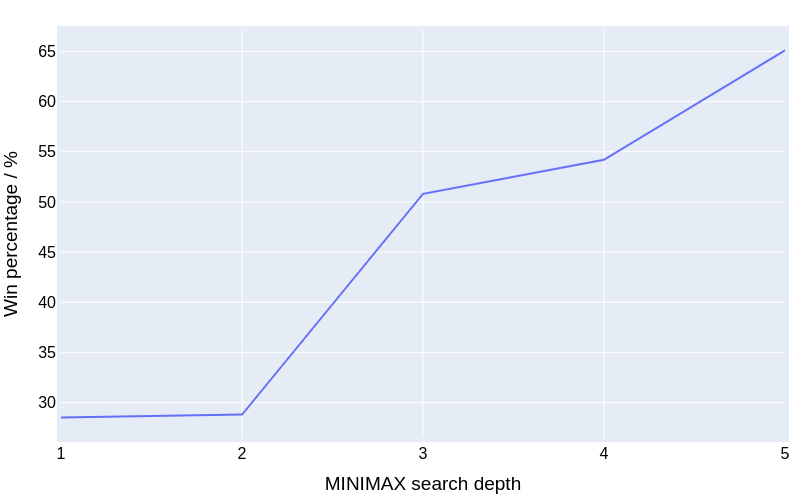
\includegraphics[width=0.8\linewidth]{plots/search_depth.png}
    \caption{Win percentage vs search depth using the baseline heuristics playing against the sample player MINIMAX algorithm with the same heuristics and a search depth of 3.}
    \label{fig:search_depth}
\end{figure}

Besides the heuristics function, the search depth of the MINIMAX algorithm has a massive impact on the win percentage. To study this is more detail, we performed various runs with our baseline heuristic while varying the search depth of our MINIMAX algorithm. In Figure \ref{fig:search_depth} we show the results.

As it is clear from this plot, the search depth is a very important influence on the win percentage. When we play with a very low search depth of 1, the win percentage falls down to 28.5\%. On the other hand, if we increase the search depth to 4 we achieve a win percentage of 54.2\%. When we go up to a search depth of 5, we already violate the time constraint of 150ms slightly in a few cases. Nevertheless, using such an high search depth gives us a win percentage of 65.1\%. Out of curiosity, we combined the search depth of 4 with our, still quite cheep, baseline + keep enemy close heuristic. With this combination, we achieved a win percentage of 56.5\%, while still staying within the time limit of 150ms at all times, which would make this our best result inside the time limit.

\section{Conclusion}

From these experiments we saw that the heuristic function is a very important part in the implementation of an adversarial agent. While already simple heuristics can when games, investigating various approaches can be very beneficial. The incorporation of cheap, already existing information, like the position of the players on the board, can lead to better heuristics and to algorithms which can perform better in tight time constraints, where increasing the search depth is no option. Choosing heuristic functions poorly, or using features which only appear to be relevant at first glance, can drastically influence the win percentage of such an agent. The winner of our heuristics comparison was by far the ``deeper'' baseline approach. A cheaper, but still good, heuristics is the baseline heuristics which tries to keep the enemy close at the same time. All the other investigated heuristics performed en par or worse than the baseline.

\section{Questions}

\subsection{What features of the game does your heuristic incorporate, and why do you think those features matter in evaluating states during search?}

While the play count would in principle be an interesting quantity to consider for deciding which heuristics to choose in which part of the game (early game vs. late game), the most interesting feature was the positions of the player and the opponent on the board. By just looking at the distance between the two players we could improve our baseline heuristics drastically. If one things about it, it also makes sense that the positions on the board matter. It is unclear, however, if following the opponent is the only good way of using this information, it turned out to be working quite well. Most likely also other heuristics based on the positions of the player and the opponent could be constructed which could help winning games, like keeping in the center of the board and could be worth an additional study.

\subsection{Analyze the search depth your agent achieves using your custom heuristic. Does search speed matter more or less than accuracy to the performance of your heuristic?}

For this we take a look at the results of our ``best'' heuristic, the ``deeper'' baseline algorithm. There we know that it is more expensive than the classical baseline heuristic. However, also with a search depth of 3 it achieves way better performance than the baseline heuristics with a search depth of 4. The search depth of 5 does beat our custom heuristic with a win percentage of 65.1\%, but, as mentioned Section \ref{sec:search_depth}, the search depth of 5 already has troubles staying below the 150ms per move. So from these experiments, my answer would be: It is worth developing a good heuristic function, even when it is a bit more costly, because it can beat just brute forcing the problem with higher search depths.

% \appendix

% \section{\label{app:some_appendix}Some appendix}

% \newpage
\bibliographystyle{unsrtnat}
%\bibliographystyle{plain}
\bibliography{references}

\end{document}